\documentclass[11pt]{article}
\usepackage[margin=1in]{geometry}
\usepackage{graphicx,booktabs,amsmath,hyperref,xcolor,caption,subcaption,microtype}
\hypersetup{colorlinks=true,linkcolor=blue!50!black,urlcolor=blue!50!black,citecolor=blue!50!black}
\captionsetup{font=small,labelfont=bf}
\newcommand{\Lstar}{L$^{*}$}
\newcommand{\ci}[2]{[#1,\,#2]}

\title{Drift to Default: Brightness Drift in Autoregressive Video Diffusion\\ Is Regression to a Prompt-Set Level}
\author{Yilin Wang\\ University of Iowa}
\date{October 2026}

\begin{document}
\maketitle

\begin{abstract}
Autoregressive (causal) video diffusion models generate long videos chunk by chunk and drift over tens of seconds:
the picture darkens, saturates or loses detail. We study this drift on Self Forcing (Wan2.1-1.3B) and LongLive with
the design tools of clinical research: paired seeds, held-out prompts, mixed-effects models, cluster-bootstrap
intervals and preregistered analyses. Across about \textbf{6{,}400} generated videos (mostly 31\,s) we find:
(i) anchoring the first frames in the KV cache (an attention sink) slows colour drift strongly, and a small rolling
window drifts fastest without it (preregistered, 2{,}000 videos);
(ii) brightness drift is \emph{two-way regression to a default level}: brighter openings darken and darker ones
brighten, only $\approx$22\% of the opening's deviation survives 31\,s, and the default is set by the text prompt
(sunny 43, overcast 34, dusk 19, night 16 \Lstar) and differs between models (33 vs 40 for the same prompt) while the
regression slope does not ($-0.69$ vs $-0.74$);
(iii) a training-free, content-aware correction that transfers the per-channel mean tone of an anchor-only prediction
at one early denoising step reduces drift without harming structure (preregistered confirmation on 40 held-out prompts)
and transfers to LongLive at half the effect;
(iv) in a preregistered test, prompts written from an off-the-shelf VLM caption of the opening did \emph{not} reduce brightness drift on either model, although they kept 0.10--0.15 more of the opening's content (DINOv2 similarity); the captioner's lighting words are poorly calibrated to actual brightness. (v) In a second preregistered test, choosing the lighting description from the opening's measured brightness, with levels taken from (ii), reduced brightness drift against the generic prompt on Self Forcing ($-26\%$, Holm $p=0.013$); combined with the correction it cut brightness drift by 44\% and colour shift by 39\%. On LongLive the effect was smaller and not significant, because the calibration was estimated on Self Forcing.
We also report what did not hold, and two evaluation pitfalls: the GPU architecture changes bf16 outputs, breaking
seed pairing, and a popular image-quality metric is insensitive to this drift.
\end{abstract}

\section{Introduction}
Causal video diffusion models such as Self Forcing~\cite{selfforcing} distil a bidirectional video diffusion model
into a student that generates a few latent frames at a time, attending to its own past through a KV cache. This makes
long, streaming generation possible and is the basis of interactive ``world models''. Over long horizons the outputs
drift. Most follow-up work proposes a fix and shows a few qualitative examples or one aggregate score from a single
sample per prompt, without uncertainty.

This report treats drift as a measurement problem. We ask three questions and answer each with a design whose analysis
plan was written down before the data existed where it mattered:
\begin{enumerate}
\item How do the two standard context strategies, a rolling window and an attention sink, affect drift? (\S\ref{sec:ctx})
\item What is drift? We find that brightness drift is regression to a default level set by the prompt, on two models. (\S\ref{sec:default})
\item Can it be reduced without training? A content-aware correction works and transfers (\S\ref{sec:corr}); describing the opening with a free-form caption does not (\S\ref{sec:match}), but a lighting description calibrated to measured brightness does (\S\ref{sec:calib}).
\end{enumerate}
No model was trained. Everything is inference on public weights, run on a university cluster. Code, prompts,
preregistrations and per-experiment summaries are at \url{https://github.com/ElaineYilinW/drift-to-default}.

\section{Setup}\label{sec:setup}
\paragraph{Models.} Self Forcing (DMD checkpoint, Wan2.1-T2V-1.3B, 4 denoising steps, chunks of 3 latent frames = 12
video frames, 16\,fps) with a rolling KV window of $w$ latent frames and $s$ permanently kept ``sink'' frames; default
$w{=}21$. LongLive 1.0~\cite{longlive} (the same base with a rank-256 LoRA, official $w{=}12$, $s{=}3$). Videos have
501 frames ($\approx$31\,s).

\paragraph{Reference-based drift metrics.} For every prompt, 10 fresh 5-second generations define the model's own
``normal'' output. \textbf{D} is the Mahalanobis distance of each frame's colour statistics (Lab means, saturation,
log sharpness) from this reference; \textbf{K} is the DINOv2 nearest-neighbour distance of a frame to the reference
frames, divided by the reference's leave-one-seed-out median (so $K\approx1$ means ``as typical as a fresh start'');
$z_L$ is the signed brightness z-score. Both D and K are averaged over the last 2 seconds. For experiments that start
from a held image, drift is measured relative to that opening: $\Delta L_\text{end}$, the change of mean \Lstar{}
between the opening (8 frames) and the last 2 seconds, and $\Delta E_\text{end}$, the Lab distance.

\paragraph{Statistics.} Seeds are paired across arms (same initial noise and random stream). Effects are estimated
with linear mixed models (random intercepts for prompt and prompt$\times$seed) or as paired differences averaged over
seeds, with prompt- or opening-cluster bootstrap confidence intervals and Holm correction for the primary family.
Three experiments were preregistered with SHA-256 hashes of the analysis code (\S\ref{sec:ctx}, \S\ref{sec:corr},
\S\ref{sec:match}); the rest is labelled exploratory.

\paragraph{A pitfall: the GPU changes the video.} With bf16, the same seed gives bit-identical videos within a GPU
architecture but different videos on A40, on A100/A800 and on L40S/RTX 6000 Ada. On a shared cluster, about 70\% of the
``paired'' comparisons in our first experiment ran on different architectures. This does not bias the comparison, but
it loses the variance reduction that pairing is meant to give. All later experiments run every arm of a prompt in one
job on one GPU.

\section{Context strategies (preregistered)}\label{sec:ctx}
We crossed window $w\in\{12,21\}$ $\times$ sink $s\in\{0,1,3\}$ $\times$ RoPE re-alignment of the sink
$\in\{\text{no},\text{yes}\}$ (10 strategies) over 40 prompts (20 MovieGen, 20 driving) $\times$ 4 seeds.
\begin{itemize}
\item Anchoring 3 frames cuts colour drift: D, sink 3 vs 0, $-7.56$ \ci{-8.32}{-6.81}; K $-0.90$ \ci{-1.04}{-0.76}.
There is a dose effect (3 $>$ 1 $>$ 0).
\item The window matters only without a sink (interaction: D $+5.71$ \ci{4.21}{7.22}, K $+0.67$).
\item Re-aligning the sink's positions, as Rolling/Deep Forcing do, did not help colour (D $-0.03$ \ci{-0.79}{0.72})
and made K worse ($+0.36$ \ci{0.22}{0.50}). Those methods were trained or designed for it; Self Forcing was not.
\item Drift is slowed, not stopped: D rises roughly linearly to 31\,s. Over-saturation disappears with a sink, but
darkening does not ($z_L<0$ in 78--88\% of anchored videos).
\item MUSIQ, the image-quality model behind VBench's imaging-quality score, is nearly flat across strategies (66--69).
It does not see this drift.
\item The seed variance of end-of-video drift was small next to the prompt variance (0.2 vs 13.7). More prompts buy
more precision than more seeds.
\end{itemize}

\begin{figure}[t]
\centering
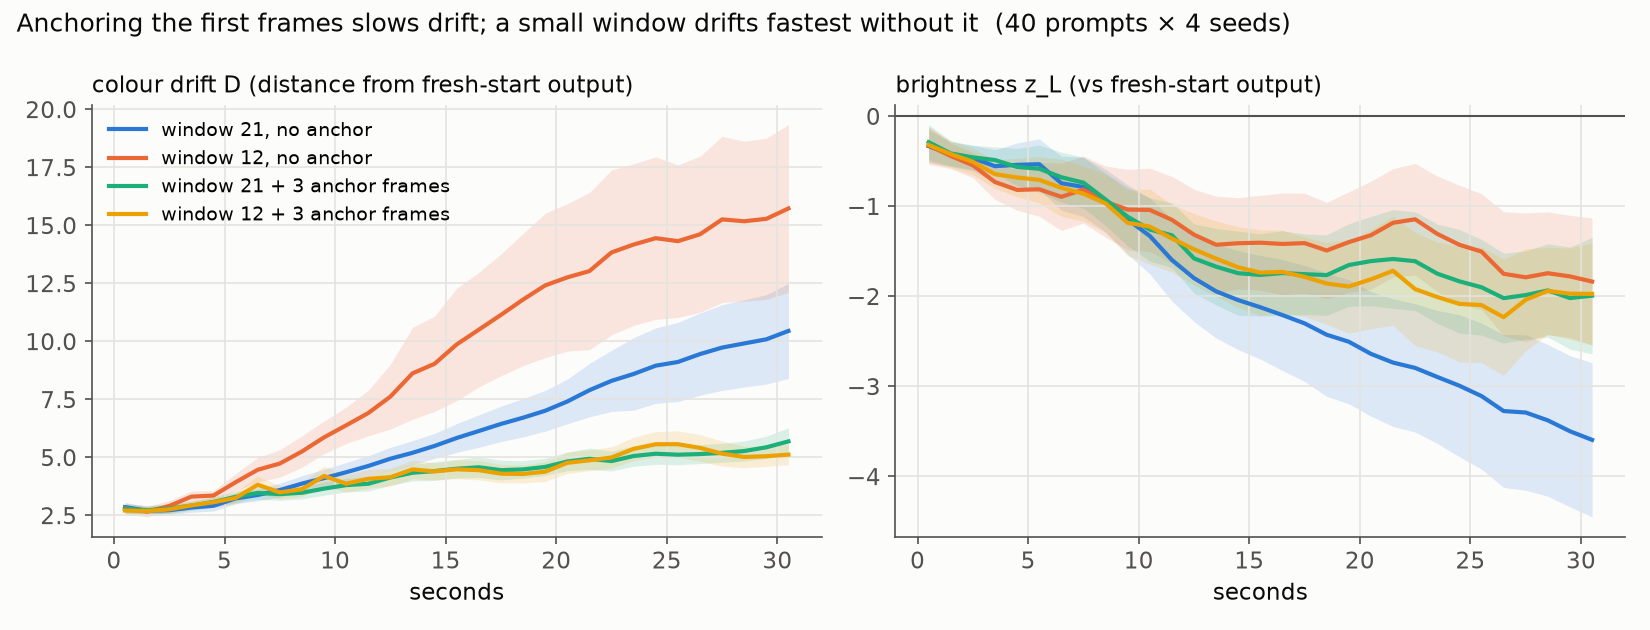
\includegraphics[width=.92\linewidth]{../assets/fig2_context_strategies.png}
\caption{Colour drift D and DINOv2 drift K at the end of 31-second videos for 10 context strategies (Self Forcing,
40 prompts $\times$ 4 seeds; means with prompt-cluster bootstrap 95\% CIs).}
\label{fig:ctx}
\end{figure}

\section{Drift is regression to a prompt-set default}\label{sec:default}
\paragraph{Held openings.} To separate drift from what the prompt asks for, we held one image for 0.5\,s as the first
chunk and let the model continue it for 31\,s with a generic driving prompt. Openings were 20 NAVSIM~\cite{navsim}
front-camera frames and 20 first frames generated by the model itself. The change in brightness is a linear function
of the opening's brightness (Fig.~\ref{fig:reg}a):
\[
\Delta L_\text{end} = 22.8 - 0.69\,L_\text{open},\qquad R^2=0.82,\quad\text{slope } \ci{-0.81}{-0.57}.
\]
Openings brighter than $\approx$33 \Lstar{} darken and darker ones brighten. Real frames darken more than generated
frames only because they are brighter (real vs generated at equal brightness: $p=0.80$). Different seeds of the same
opening move towards a common level; an early deviation persists only 10--30\%.

\paragraph{The prompt sets the level.} We continued the same 40 openings under four prompts that differ only in
their lighting description (320 videos, exploratory). Each prompt pulls the video to its own level
(Fig.~\ref{fig:reg}b): zero-drift levels are 42.9 \ci{41.0}{44.7} (sunny), 33.6 (overcast; the generic prompt: 33.1),
19.1 (dusk) and 16.0 \ci{12.5}{19.9} (night). In a joint model the lighting term is overwhelming ($p\approx5\times10^{-78}$,
$R^2$ 0.82\,$\to$\,0.90) and the common slope is $-0.78$ \ci{-0.83}{-0.72}: after 31 seconds only about a fifth of
the opening's brightness deviation is left. Darker prompts regress more completely (slope $-0.95$ for night vs $-0.66$
for sunny; interaction $p=0.011$). For dusk and night the prompt may legitimately ask for a darker scene, so these
levels describe the prompt's target, not a defect.

\paragraph{Second model.} On LongLive the same openings regress with the same slope ($-0.74$ \ci{-1.01}{-0.58};
model$\times$slope $p=0.59$) to a brighter default (39.9 \ci{37.5}{42.1}; $R^2=0.65$; Fig.~\ref{fig:reg}c). LongLive
seemed hardly to darken real driving frames (mean 47 \Lstar) because they start closer to its default, not because
it regresses less. Unlike Self Forcing, LongLive darkens real openings 4.3 \Lstar{} more than generated ones of equal
brightness ($p=0.03$).

\paragraph{Interpretation.} Over a long rollout the model forgets the opening and returns to what the text
describes. ``Colour drift'' in this sense is a conflict between the visual context and the text condition that the
text wins. This matters for world models that start from real camera frames and a caption.

\begin{figure}[t]
\centering
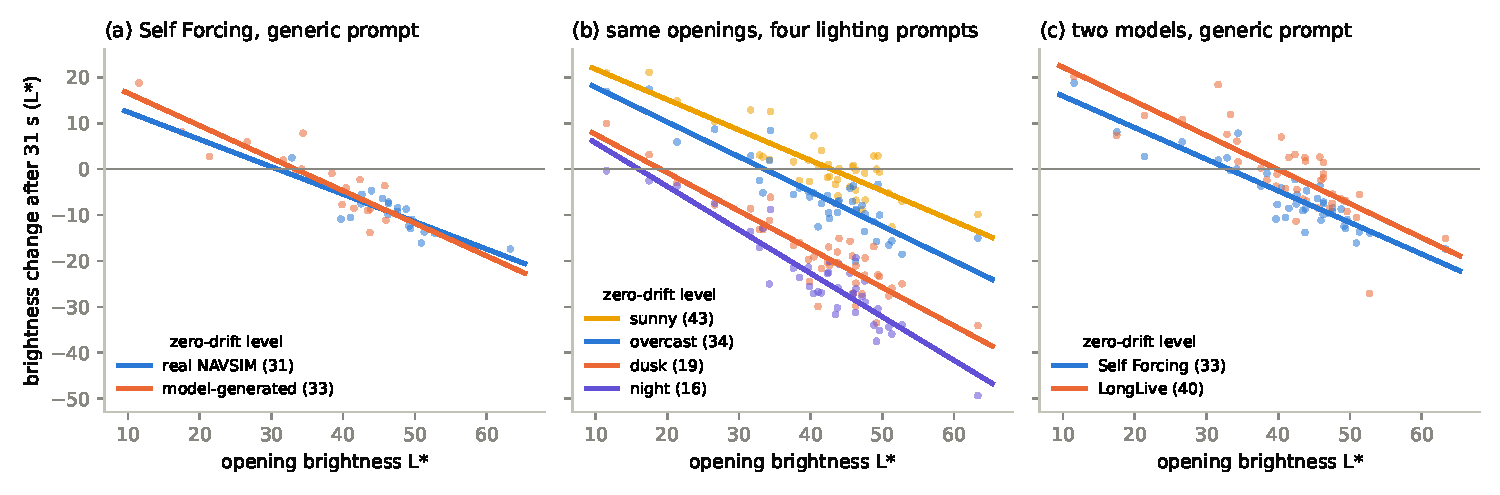
\includegraphics[width=\linewidth]{fig_default.pdf}
\caption{Brightness change after 31\,s against the brightness of the held opening; one dot per opening (mean of
seeds), lines are least-squares fits, legend gives the zero-drift level $-a/b$. (a) Self Forcing with the generic
prompt; real and generated openings fall on the same line. (b) The same openings under four lighting prompts. (c) Self
Forcing vs LongLive: same slope, different default.}
\label{fig:reg}
\end{figure}

\section{A training-free correction}\label{sec:corr}
\paragraph{What failed.} A statistical closed-loop brightness controller (integral control with a jump guard and a
CUSUM trigger) could not tell legitimate dimming from drift: it lifted tunnels to over-exposure, and its jump guard
ratcheted on its own corrections. A regression-derived ``brightness direction'' in latent space realised only 18\% of
an intended change; a direction estimated from designed per-channel perturbations realised 96\%. Observational
estimates gave the wrong causal answer here.

\paragraph{Content-aware correction.} At denoising step 1 of 4, the same noisy chunk is run once more with a temporary
KV cache that holds only the clean anchor frames. The difference between the per-channel spatial means (the ``DC''
tone of each of the 16 latent channels, per frame) of that prediction and of the real prediction is added, scaled by
$\beta$. Layout and detail are untouched, and so are the main KV cache and the random stream. It costs one extra
forward pass per chunk. The denoising step is a knob between drift removal and content fidelity: correcting at step 0
removes most drift but erases legitimate transitions such as entering a tunnel (56\% kept), step 1 keeps 92\%, and
steps 2--3 have no effect.

\paragraph{Confirmation (preregistered).} On 40 held-out prompts $\times$ 4 seeds, on one GPU architecture, every
criterion was met: D $-1.48$ \ci{-1.76}{-1.19} ($\beta{=}1$) and $-1.78$ \ci{-2.11}{-1.45} ($\beta{=}1.5$); $z_L$ +1.08
and +1.32; K non-inferior (difference $\approx0$, CI $\pm0.11$); held-out control prompts with legitimate brightness
changes kept a median 83\% / 93\% of their transition. Flicker is the cost: jitter $\times$1.13 / $\times$1.67 and
chunk-boundary jumps $\times$1.32 / $\times$2.40. On held real openings, the colour shift from the opening fell from
10.7 to 8.1 / 7.8 \Lstar{} without more flicker.

\paragraph{Transfer to LongLive (exploratory).} Ported without changes, the correction reduces D by 0.70
\ci{-1.13}{-0.27} on the 40 main prompts (2 seeds), keeps structure (K $+0.05$ \ci{-0.10}{0.20}) and adds little
flicker ($\times$1.10). On held openings $|\Delta L_\text{end}|$ falls from 7.4 to 5.2 (30/40 scenes improved). The
effect is about half that on Self Forcing because LongLive darkens less on these prompts ($z_L$ $-0.67$ vs $-2.19$);
$\beta{=}1.5$ brings no further gain.

\begin{figure}[t]
\centering
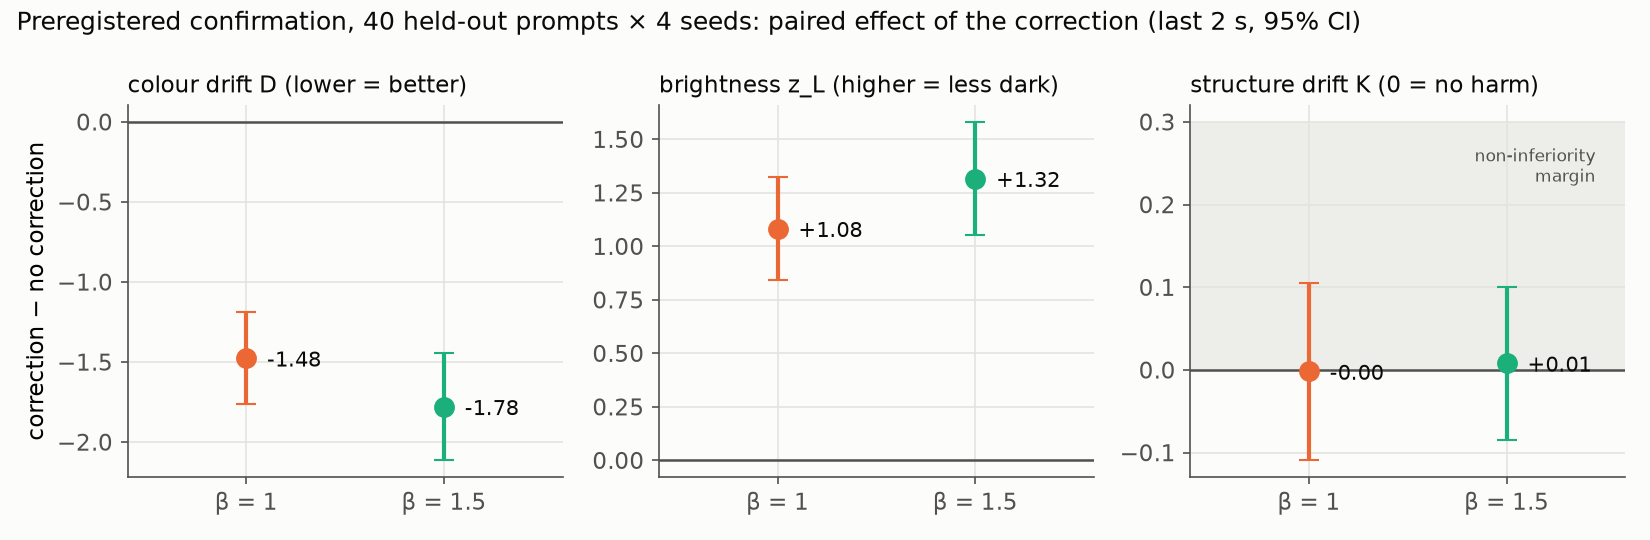
\includegraphics[width=.8\linewidth]{../assets/fig3_correction_confirmatory.png}
\caption{Preregistered confirmation of the correction on Self Forcing: paired effects on 40 held-out prompts
$\times$ 4 seeds with prompt-cluster bootstrap 95\% CIs.}
\label{fig:corr}
\end{figure}

\section{Matching the prompt to the opening (preregistered)}\label{sec:match}
\paragraph{Design.} If drift is the text overriding the opening, a prompt that describes the opening should drift
less. We froze the analysis, the openings and all prompts before generating any video (public commit 43bbd4c). The 40
new openings are 20 NAVSIM frames from logs not used before, chosen evenly over brightness (15.6--60.7 \Lstar), and 20
new model-generated first frames. For each opening, Qwen2.5-VL-3B-Instruct (greedy decoding) wrote a scene phrase and
a lighting sentence. Three prompts were built: the generic prompt (G); scene + lighting from the caption (M); and the
generic scene with the caption's lighting sentence only (ML). G and M were run with and without the correction, ML
without, on both models with 2 seeds: 800 videos, all arms of an opening on one GPU. Primary hypotheses: $|\Delta
L_\text{end}|$ is lower for M than G (H1) and lower for M+correction than M (H2), on each model, Holm-corrected over the
four tests.

\paragraph{Primary result: not supported.} H1: $-1.21$ \ci{-3.09}{0.36} on Self Forcing (Holm $p=0.58$) and $-0.19$
\ci{-2.00}{1.63} on LongLive. H2: $-1.00$ \ci{-1.89}{-0.12} on Self Forcing (nominal $p=0.035$, Holm $p=0.14$) and
$-0.36$ \ci{-1.48}{0.75} on LongLive. Captioning the opening with an off-the-shelf VLM does not reliably reduce
brightness drift (Fig.~\ref{fig:match}a).

\paragraph{Secondary results.} The caption prompt strongly improves \emph{content} retention, the DINOv2 cosine
similarity between the last 2 seconds and the opening: $+0.10$ \ci{0.06}{0.14} on Self Forcing (0.40\,$\to$\,0.50) and
$+0.15$ \ci{0.10}{0.21} on LongLive (0.40\,$\to$\,0.56) (Fig.~\ref{fig:match}b). It also lowers jitter ($\times$0.79,
$\times$0.71). On Self Forcing, caption prompt plus correction vs the generic prompt reduces $|\Delta L|$ by 2.21
\ci{-3.99}{-0.56} and the colour shift $\Delta E$ by 2.93 \ci{-4.83}{-1.20}. The lighting sentence alone (ML) does
nothing for brightness.

\paragraph{Why (exploratory).} Grouping openings by the lighting words of their caption shows the mechanism of
\S\ref{sec:default} at work, with a miscalibrated input (Fig.~\ref{fig:match}c). The captioner called half of the
normally lit frames ``dimly lit, likely early morning or late evening'' (mean 40 \Lstar, up to 61). For these frames
the caption prompt made Self Forcing darken \emph{more} ($-5.6\to-8.7$; ML $-11.2$). For the 4 frames captioned as night
or very dark (mean 21 \Lstar), the generic prompt brightened them by 16 \Lstar{} and the caption prompt kept them
($-2.9$). The prompt does set the level, but a free-form caption does not say how bright the scene is. A lighting
description calibrated to measured brightness is the natural next test; with only 4 dark openings, this breakdown is a
hypothesis, not a finding.

\begin{figure}[t]
\centering
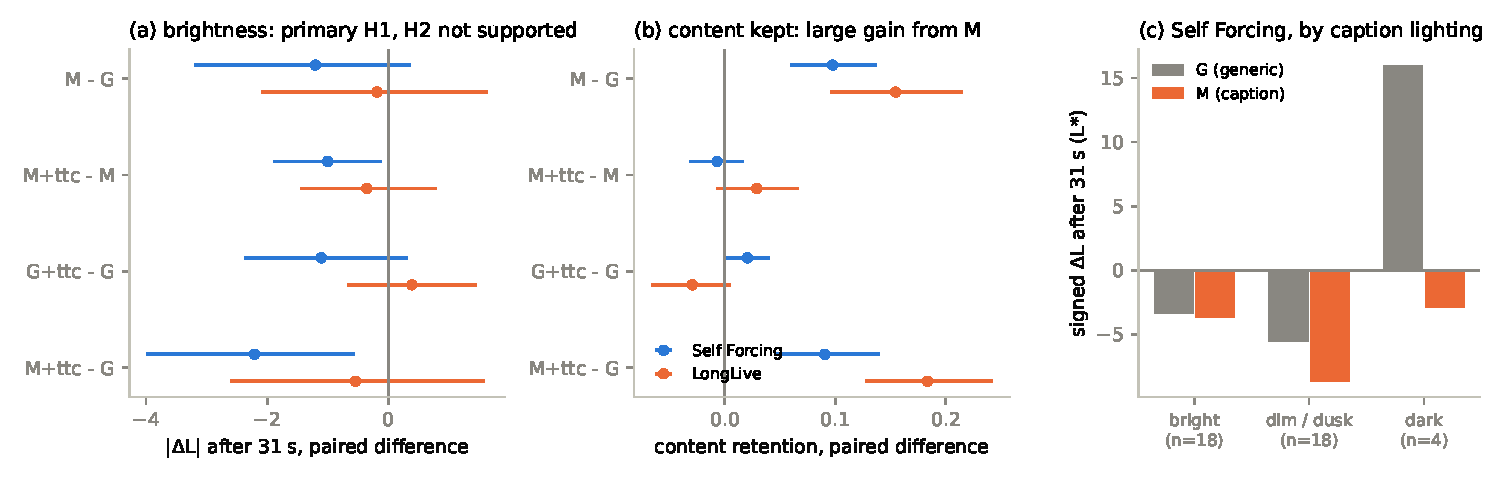
\includegraphics[width=\linewidth]{fig_match.pdf}
\caption{Matched-prompt experiment (40 new openings $\times$ 2 seeds per model). (a, b) Paired differences between arms
with opening-cluster bootstrap 95\% CIs. (c) Exploratory: signed brightness change on Self Forcing by the lighting
words of the VLM caption.}
\label{fig:match}
\end{figure}

\section{Calibrating the lighting description (preregistered)}\label{sec:calib}
\paragraph{Design.} If the failure in \S\ref{sec:match} comes from the caption's lighting words, choosing those words
from measured brightness should work. We froze the rule before generation (public commit d5e4c24). Each opening gets the
Part~4 lighting prompt whose Self Forcing zero-drift level is nearest to its brightness (night 16, dusk 19, overcast 34,
sunny 43; levels estimated on the earlier, independent openings). This gave 23 sunny, 10 overcast, 5 dusk and 2 night.
New arms: CL (generic scene + calibrated lighting, i.e.\ the Part~4 prompt itself), C (the VLM scene phrase +
calibrated lighting) and C+correction. They were compared with the existing G and M videos of \S\ref{sec:match}. Each
opening ran on the GPU architecture of its earlier arms. A rerun of G (seed 0) reproduced all 80 stored videos bit for
bit, so the new and old arms are strictly paired. While preparing this run we found that 4 LongLive openings of
\S\ref{sec:match} had arms split across architectures (a preempted job resumed on another GPU type). We regenerated
them; the preregistered conclusions of \S\ref{sec:match} did not change. Primary hypotheses, per model and
Holm-corrected: $|\Delta L_\text{end}|$ lower for C than M (H1) and lower for C than G (H2).

\paragraph{Results.} H2 is supported on Self Forcing: $-2.45$ \ci{-4.08}{-1.04} (9.29\,$\to$\,6.84, Holm $p=0.013$).
H1 points the same way on both models ($-1.24$ and $-1.15$) but is not significant, and neither is H2 on LongLive
($-1.34$ \ci{-3.19}{0.55}). Secondary results (Fig.~\ref{fig:calib}):
\begin{itemize}
\item On Self Forcing, the plain calibrated prompt CL reduces $|\Delta L|$ by 3.20 \ci{-4.69}{-1.89}.
\item Calibrated prompt + correction vs generic reduces $|\Delta L|$ by 4.05 \ci{-5.64}{-2.54} (44\%) and $\Delta E$ by
4.54 (39\%). Content retention improves (+0.08) and jitter falls.
\item Content retention comes from the VLM scene phrase (C vs CL: +0.06 on Self Forcing, +0.14 on LongLive), not from
the lighting words.
\item The Part~4 law, applied out of sample, predicts the CL outcomes on Self Forcing moderately (correlation 0.64,
$R^2$ 0.34).
\item On LongLive the same predictions are biased by $+4.3$ \Lstar: its defaults are higher, so dark openings were
still brightened under the Self-Forcing-calibrated prompts. A calibration has to be estimated per model.
\end{itemize}

\begin{figure}[t]
\centering
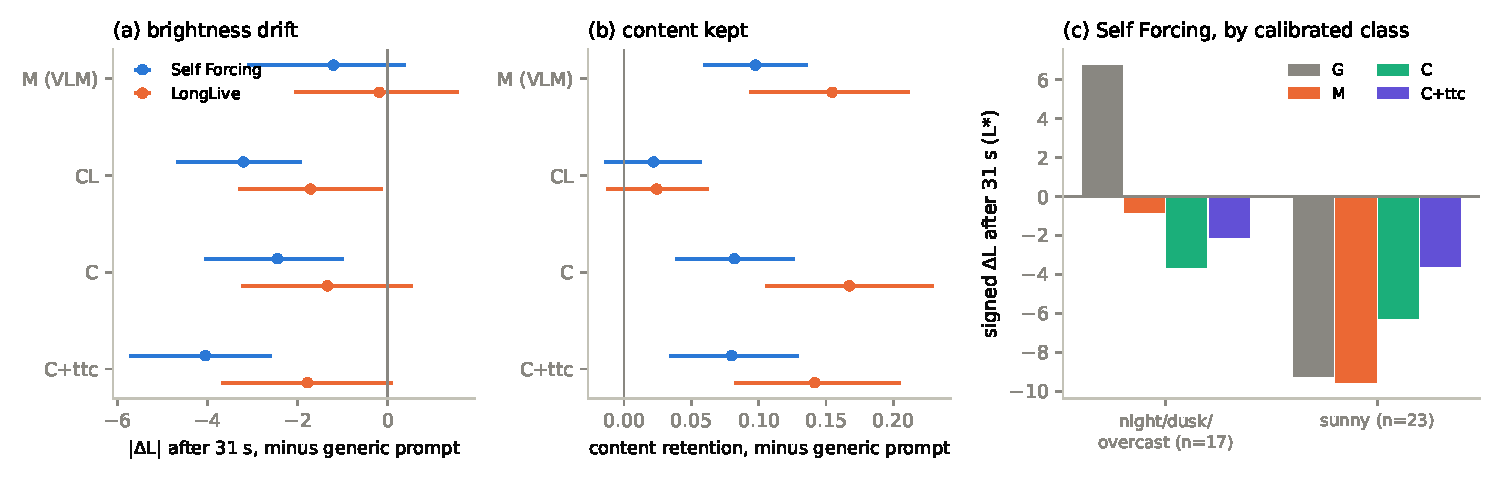
\includegraphics[width=\linewidth]{fig_calib.pdf}
\caption{Calibrated lighting descriptions. (a, b) Paired differences from the generic prompt (40 openings, seed means,
opening-cluster bootstrap 95\% CIs). (c) Self Forcing, signed brightness change by calibrated class.}
\label{fig:calib}
\end{figure}

\section{What did not hold}
We report claims that we made at some point during the study and later revised or withdrew after further checks:
\begin{itemize}
\item \emph{``MUSIQ rewards collapsed videos.''} Seen in the pilot, not replicated in the main experiment: MUSIQ is
simply insensitive.
\item \emph{``The sink works by stabilising the default level.''} Withdrawn: the trend difference was $+0.5$
\ci{-2.4}{3.5}.
\item \emph{``The model follows its recent context about 75\%.''} True only for an artificial tone shift. For natural
differences (swapping in another seed's window by KV-cache replay, bit-exact) it follows 90--100\%. The sink frames
have a direct effect of only 0.036, yet they reduce drift; how is not explained.
\item \emph{A dynamics model that forecasts the final brightness of a video.} Out-of-sample forecasts were weak.
\end{itemize}

\section{Limitations}
Both models share the Wan2.1-1.3B base. The preregistered positive results are on Self Forcing; of the two preregistered tests on both models, the first (\S\ref{sec:match}) was negative and the second (\S\ref{sec:calib}) positive on Self Forcing only. The lighting calibration has four discrete levels and was estimated on Self Forcing; openings brighter than the sunny level (43 \Lstar) have no matching description. The lighting
and LongLive experiments use 2 seeds. Videos are 31 seconds. Real openings are single held frames, not real video. The
correction acts on colour and brightness only; structural degradation (for example sky textures late in a video)
remains.

\section{Related work}
Self Forcing~\cite{selfforcing} and its long-video successors (Self-Forcing++, LongLive~\cite{longlive}, Rolling
Forcing, Deep Forcing~\cite{deepforcing}) use rolling windows, sinks and re-aligned positions; we measure these choices
with uncertainty. Pathwise test-time correction~\cite{pathwise} and FreqForcing~\cite{freqforcing} correct drift at
inference; our correction is a simplification (DC-only transfer at one early step) studied with a preregistered
confirmation. Meta-ARVDM~\cite{metaarvdm} analyses error accumulation theoretically.

\begin{thebibliography}{9}\small
\bibitem{selfforcing} X. Huang et al. Self Forcing: Bridging the train-test gap in autoregressive video diffusion. arXiv:2506.08009, 2025.
\bibitem{longlive} S. Yang et al. LongLive: Real-time interactive long video generation. NVlabs, 2025.
\bibitem{deepforcing} Deep Forcing. arXiv:2512.05081, 2025.
\bibitem{pathwise} Pathwise test-time correction for autoregressive video diffusion. arXiv:2602.05871, 2026.
\bibitem{freqforcing} FreqForcing. arXiv:2607.27110, 2026.
\bibitem{metaarvdm} Meta-ARVDM. arXiv:2503.10704, 2025.
\bibitem{navsim} D. Dauner et al. NAVSIM: Data-driven non-reactive autonomous vehicle simulation and benchmarking. NeurIPS 2024.
\end{thebibliography}
\end{document}
